\begin{flushleft}
	
	\titleformat {\chapter} {\normalfont\huge\bfseries\color{black}}   {\thechapter}{10pt}{\huge} 
	\chapter {System Architecture }	
	
	\section{Cassandra Database Cluster Architecture Design}
	
	
	\vspace*{1\baselineskip}
	\begin{figure}[htbp]
		\begin{center}
		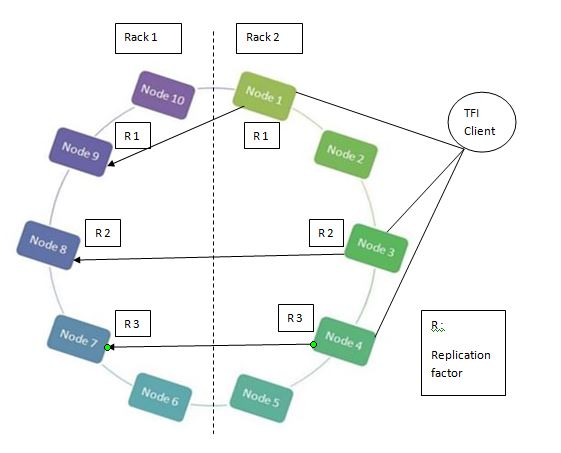
\includegraphics[width=1.00\linewidth]{./images/lala.jpg}
		\caption{Cassandra database cluster for Tank Farm Inventory System.}
		\label{fig:lala.jpg}
		\end{center}
	\end{figure}
		
	
	
	\subsection{Description}
	\vspace*{1\baselineskip}
	\noindent{
		Based on figure 3.1,The cassandra database architecture design consist of 2 racks of cassandra database cluster, with each rack comprising of 5 compute-nodes.Besides that,It also design with a replication factor of 3.TFI client connects to the main node then the main node continues jumping to the other random nodes as a copy until the 3rd copy then it stops and transfer back to TFI client.\\}
	
	
\end{flushleft}